% flotsam.tex
%
% Predrag created file				jun 20 2006

\section{Flotsam}


\subsection{Vaggelis gonne fishing for Davidchack's KS box {\rpo s}}

Full space KS, $L=22$.

\subsubsection{Equilibrium A (and its symmetric partner SA)}

Equilibrium A eigenvalues of $\Mvar$:

$(\Lyap_i \pm \theta_i)
=(
  0.139 \pm i 0.238,
 -0.084 \pm i 0.160,
 -0.271 \pm i 0.356,
\cdots
)$

The equilibrium point is accurate to at least to $10^{-11}$. Since
Lapack is also double precision accurate, the accuracy of the first
few eigenvalues is similar, and certainly in
excess of 6 significant digits.



For a numerical check of the \rpo\ stability eigenvalues,
used two inital
points along an unstable eigenvector $\jEigvec{1}$
at radial distance  $\approx 10^{-4}$ from the equilibrium A,
and the initial inter-point separation $\Delta(0) \approx 10^{-5}$.
Integrated for time equal to the period $T=26.3556$ as calculated from
the \jacobianM\ and computed the leading Lyapunov exponent from the ratio of
final to initial distance 
$\Lyap= {1 \over T}\ln( \Delta(T)/\Delta(0))$.
Get
$\Delta(T)/\Delta(0) =39.01$,
$\Lyap=0.13902$, in agreement with the equilibrium point A 
expanding eigenvalue $\Lyap=0.13904$
\[
\ExpaEig_{radial} =  e^{\Lyap T} =38.99
\,.
\]

\underline{Need to trace out}
the unstable manifold plane, like Gibson did for plane Couette.

By symmetry there might be an equilibrium on the reflection plane that
relates the equilibrium A and its symmetry partner SA; the 3 equilibria would
be analogous to what you see in the Lorentz attractor pictures, crossing
the unstable manifold of the central one throws you into the neighborhood
of the other equilibrium.

\underline{Next step}: try to find the equilibrium that corresponds to fitting
exactly 3 complete periods of $u(x)$ into interval $L$.
Orbits coming close to this one
show up in Davidchack's \rpo s.

\subsubsection{\Reqva}

\underline{Need to detemine} important {\Reqva} (traveling waves).

\subsubsection{\Rpo s}


The \rpo\ [NAME IT] travels between the equilibrium A and its symmetric partner SA 
with period and shift
$T=55.6, d=5.25$
Compared to $L/4 = 5.5$
this is nice, but why not close to periodic after 2nd return? Why 4th return?

%  Eigenvalues of the Jacobian without rotation
%  84.15, -33.86 + 28.94 i, c.c. , 0.48, 0.00019
% no good - missing marginal ones

Eigenvalues of \rpo\ [NAME IT] $g\jMps$: are
$ -57.17,  1.00009, 1.00001, -0.500, -0.012, \cdots$ .
This all makes sense: The period is roughly double of the rotation period of
the equilibrium point, as the trajectory makes a figure 8 around equilibrium A and
its symmetric partner SA.
 There are two
marginal eigenvalues, one for time translation, one for
circle translation. 
The sign of $\ExpaEig_{1}=-57$ says this is a Moebius-kind orbit,
inverse hyperbolic, presumably due to the symmetry relating A and SA.
Lyapunov $\Lyap=0.07$ says that this neighborhood is much less repelling than
the central equilibrium A, a better candidate for being embedded into the
ergodic attractor.

For the \rpo s the accuracy of Jacobian depends
on the time step size, and long runs are needed to refine the results
We check by redoing the caluclation with double 
number of Fourier modes, observe how many digits
change. 
Because of the strong contractionin KS we expect at most 10 eigenvalues to be
significant, rest are in the numerical noise. See figure~6 in
\refref{Christiansen:97}.
Stated here are only the digits we trust.


I've reread parts of ``Discrete symmetries" chapter - not an easy read, but
it also uses $g\jMps$ rather than the naked $\jMps$, and a trace formula for irrational
$d/L$ still puzzles me - for $d/L$ rational the determinant factorizes using
discrete Fourier transform.

\subsection{{\Rpo s} in classical mechanics}

Chenciner\rf{ChencinerLink}
says Poincar\'e introduced them in the 3-body problem.
Consider motion of a test particle of mass
$\mu \ll 1$ in the
restricted three-body problem\rf{rtb},
under the
influence of the gravitational force of two heavy bodies with masses $1$ and
$\mu \ll 1$ fixed at $(-\mu,0)$ and $(1-\mu,0)$. \Reqv\ of this problem
(known in this context as the Lagrange points, stationary in
the co-rotating frame) are circular motions in the inertial frame,
and {\rpo s} correspond to quasiperiodic motions. 

%%%%%%%%%%%%%%%%%%%%%%%%%%%%%%%%%%%%%%%%%%%%%%%%%%%%%%%%%%%%%%%%
\begin{figure}[t] %[h]
\centering
(c) 
\includegraphics[width=2.5cm]{figs/path.eps}
\hspace{0.1in}
(b) 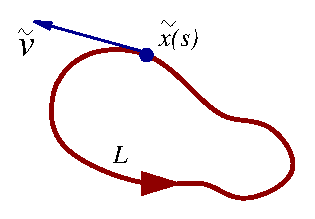
\includegraphics[width=3.5cm]{figs/loop.eps}
\hspace{0.1in}
(c) 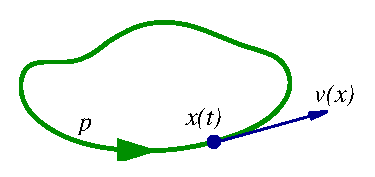
\includegraphics[width=4.0cm]{figs/porbit.eps}
\caption{
 (a) A continuous path; (b) a loop $\Loop$ with its tangent velocity vector $\lVeloc$;
 (c) a periodic orbit $p$ defined by the vector field $\pVeloc(\pSpace)$.
        }
\label{f:loops}
\end{figure}
%%%%%%%%%%%%%%%%%%%%%%%%%%%%%%%%%%%%%%%%%%%%%%%%%%%%%%%%%%%%%%%%%%

    In order to set the notation, we shall distinguish between (see \reffig{f:loops}):

\medskip
\noindent
 {\bf closed path:}
 any closed (not necessarily differentiable) continuous curve 
$J \subset \pS$.

\medskip
\noindent
{\bf loop:}
 a smooth, differentiable closed curve $\lSpace(s)\in \Loop \subset 
\pS$, 
parametrized by $s \in [0,2\pi]$ with $\lSpace(s)=\lSpace(s+2\pi)$, with the
magnitude of the loop tangent vector fixed by 
the (so far arbitrary) parametrization of the loop,
\[
\lVeloc(\lSpace)=\frac{d \lSpace}{ds}\,, \quad \lSpace=\lSpace(s) \in \Loop
\,.
\]   
{\bf annulus:} 
 a smooth, differentiable surface $\lSpace(s,\tau)\in \Loop(\tau)$ swept by a 
family of loops $\Loop(\tau)$, by integration along a fictitious time flow
(see \reffig{f:velocField}~(a))
\[
\dot{\lSpace}=\frac{\partial \lSpace}{\partial \tau}
\,.
\]
{\bf periodic orbit:}
 given a smooth vector field $\pVeloc=\pVeloc(\pSpace),\; (\pSpace,\pVeloc) \in {\bf T} \pS$, periodic orbit $\pSpace(t) \in p$ is a solution of
\[
\frac{dx}{dt}=\pVeloc(\pSpace) 
	\,,\quad
	\mbox{ such that } \pSpace(t)=\pSpace(t+\period{p}),
\] 
where $\period{p}$ is the shortest period of $p$.



The strategy
is to minimize an action functional defined on a space of paths $\gamma$ in the
configuration space $\pS$ which satisfy the property
\beq
                               \gamma (t + T ) = g \cdot \gamma (t)                       
\label{McC1}
\eeq
for a fixed {\em relative period} $T$ and some fixed diffeomorphism $g$ of $\pS$, 
sometimes referred to as a {\em phase}, that leaves the 
action functional invariant. If $g^k=1$ is of finite order
$k$, then the corresponding orbit is periodic with period $k T$. 

Striking applications of this idea has been the discovery
of ``choreographies" of $N$-body problems\rf{McC7,McC8,McC}.
\PC{some McCord references}

If $g$ does not have finite order $k$, the
paths can be periodic after the action of $g$. 
In either case, order we refer to the loops
in $\pS$ satisfying \refeq{McC1} as 
{\em relative loops} and
to the corresponding solutions of the equations of motion
as {\em \rpo}. 

    Let $A[\gamma]$ be an action functional defined loops $\Loop$
emebedded in the state space manifold $\pS$, invariant
under a diffeomorphism $g : \pS \to\pS$. Our aim is to determine
the critical points of the action functional
$ %\beq
	A[\gamma]
  % =\int_0^T  dt L(\gamma,\dot\gamma, t)
$ % \label{McC2}
  % \eeq
defined on $\Lambda_g^1(\pS)$, a Sobolev space of paths in $\pS$ satisfying 
\refeq{McC1}.
\PC{define Sobolev space as adding a vector space?}


\subsection{V. Lopez: 
	    {\Rpo s} of the Complex Ginzburg-Landau Equation}

        John, Jonathan, Vaggelis and Rytis have been pondering role of
continuous symmetries (simple ones - translations, periodic domains) in
periodic orbit theory. One needs to
generalize notion of ``periodic" to ``relative periodic" (equvariant,
travelling, running are other names I have heard), and recently
we have received results from Viswanath (who finds such in plane Couette)
and Davidchack (who finds such in Kuramoto-Sivshinsky on a periodic
domain).

As far as the discussion about ``drift" is concerned:
In presence of continuous symmetries (for PC, streamwise and
spanwise translations) one should be searching for 
{\reqva} and 
{\rpo s} - they are most likely more important than
the stationary equilibria and spatially periodic orbits. 

I like {\rpo s} paper\rf{lop05rel} by
Vanessa Lopez\rf{lopezLink},
%        http://www.cse.uiuc.edu/$\sim$vlopez:
``Relative Periodic Solutions of the Complex Ginzburg-Landau Equation" 
     
We have such systems whenever we have a translational symmetry (like plane
Couette).
{\Rpo s} were missed in earlier 
previous Kuramoto-Sivashinsky investigations%
\rf{Christiansen:97,Lan:Thesis}
which focused on the antisymmetric subspace, where translational invariance
is broken.

% [From siads\@siam.org  Dec 22 2004]:
% willing to review this manuscript for Dwight Barkley.
     
A method of finding {\rpo s} for differential equations with 
continuous symmetries is described and its utility demonstrated by computing 
{\rpo s} for the one-dimensional complex Ginzburg-Landau 
equation (CGLE) with periodic boundary conditions.  A {\rpo} is 
a solution that is periodic in time, up to a transformation by an element of the 
equation's symmetry group.  With the method used, {\rpo s} are 
represented by a space-time Fourier series modified to include the symmetry 
group element and are sought as solutions to a system of nonlinear algebraic 
equations for the Fourier coefficients, group element, and time period. 
{\Rpo s} found for the CGLE exhibit a wide variety of temporal 
dynamics.
with the % sum of their positive Lyapunov exponents varying from 5.19 to 
% 60.35 and their
unstable dimensions from 3 to 8.
% Preliminary work indicates that 
% weighted averages over the collection of {\rpo s} accurately 
% approximate the value of several functionals on typical trajectories.

15 Sep 2004, Predrag Cvitanovic:
* All of your {\Rpo s} have many unstable
eigendirections. Do you know that there exist no other solutions with a
lesser number of unstable directions (let's say only one)?

--vanessa:
I do not know of any proof that shows that there are no solutions with a
lesser number of unstable directions.  I did not find any solutions with
just one or two unstable directions, but at this point I cannot say
whether that is an indication that there are none or simply that (for some
 to
be able to analyze full-space Kuramoto-Sivashinsky 
reason) the procedure I used only identified solutions with 3+ unstable
directions.

15 Sep 2004, Predrag Cvitanovic:
* Periodic solutions are usefull if they are embedded into a chaotic
attractor. Do you have any measure of whether the typical solutions of
CGL, your parameter values, come close to any of the solutions that you
have found? If the periodic orbit is embedded into a chaotic attractor,
typical soultion visits it infinitely often, infinitesimally close.

--vanessa:
This is something that I have not examined in detail.  I have observed (using
the ``naked eye") that the time evolution of typical trajectories (when viewed
by plotting the real versus imaginary part of A(x,t) at different times, as in
Figures 3,5,7 from the paper) sometimes resembles that of the first solution
found (i.e., the patterns displayed in Figure 3). (The first solution
found also happened to be the solution to which the solver I used
converged to most frequently.)  But at this point I do not have a
quantitative measure of this ``resemblance".

After talking to Lopez at SIAM DS05 meeting - she did something that
is useful to us (found some {\rpo s}), but I do not think
they are the dynamically important ones, so the problem remains wide open.

I read through
Vanessa Lopez's paper (clearly a summary of a PhD thesis), and while I
a like {\rpo s}, I am very worried about the general drift
of the paper.

As I cannot tell how exhaustive is her set of numerical solutions, I do
not know what to make of them - like ZG, she gets all of them with a large
number unstable dimensions. Presumably none of them are close to the
asymptotic inertial manifold. More worrisome still, she uses ZG to
``average" over periodic orbits. That is regrettable - I hoped I would
never see that stuff again. Dettmann and I tried to get Zoldi to
derive this for us, and Mainieri actually hired him at Los Alamos to learn
how this works. We are all convinced that it makes no sense whatsoever.
Regrettably Lopez used the nonsensical formulas of Zoldy, so that will
just keep confusing future readers. 
She is in computer science, so cannot
blame a graduate student for trying a formula published in Phys Rev Lett.


If she is right and CGL at her parameter values does not contain
(relative) periodic orbits with 1 or very few unstable directions, we can
kiss the ``minimal instability principle" goodbye.

The 
periodic orbits
did not captured the main dynamics of the system. In fact, in the full
space I believe that the {\rpo s} are the more commonly
encountered objects in the phase space, just as the quasi-periodic motion is a
more frequent occurrence on an invariant torus. In a system with continous
symmetry, any orbit corresponds to a continous family of orbits, so the KS
system with periodic boundary condition is born on some kind of torus. We can
either reduce the system so that the continuous symmetry does not exist, or
study {\rpo s}. {\Rpo s} correspond to periodic
orbits in the reduced system. I don't know how to reduce the KS system in a
pretty way.

      In the case of {\rpo s}, we can find a piece of orbit on
the torus and construct the whole torus by a {\em known}
global symmetry operation in the
state space. For a generic torus solution, we do not have 
a global symmetry. 

        I am confused, and on odd days of the week I
 believe that generically such solutions are quasiperiodic.

        Here we discuss these continuous symmetries as
a small-step limit of discrete symmetries:

\begin{enumerate}
\item
        symmetries of 3-disk
\item
        $C_n$ symmetry of $n$-slice pizza without reflection symmetry
\item
        Fourier analysis of periodic lattices
\item
        running modes in periodic lattice deterministic
           diffusion
\item
	celestial {\rpo s}
\end{enumerate}

The reading material for 1)-3) is on
http://www.cns.gatech.edu/courses/chaosSpring06

In my Kuramoto-Sivashinsky work with Christiansen, Putkaradze and Lan we
had excluded them ``by hand", by concentrating only on the space of
antisymmetric solutions. That is not good physics, as perturbations off
them mix into the full space of asymmetric solutions. One part of our
proposed FRG would be a search for {\rpo s} of
Kuramoto-Sivashinsky, with my student Evangelos Siminos.

\subsection{F Laurent-Polz: {\Rpo s} in point vortex systems}

We give a method to determine {\rpo s} in point vortex systems: it consists mainly into perform a symplectic reduction on a fixed point submanifold in order to obtain a two-dimensional reduced phase space. The method is applied to point vortices systems on a sphere and on the plane, but works for other surfaces with isotropy (cylinder, ellipsoid, ...). The method permits also to determine some 
{\reqva} and heteroclinic cycles connecting these {\reqva}.

    {\Reqva} are orbits of the symmetry group action which are in-
variant under the flow, this corresponds here to motions of point vortices which
are stationary in a steadily rotating frame. We first review the literature about
the point vortex system on the sphere. The existence and nonlinear stability
of {\reqva} formed of three vortices have been studied respectively in
[KN98] and [PM98]. 

    {\Rpo s} are the analogs of {\reqva}
- concerning periodic orbits, this corresponds here to motions which are
periodic in a steadily rotating frame (a precise definition is given in Section
2). Periodic orbits on the sphere were determined in [ST, To01] thanks to the
following method: they reduced the system to two-dimensional systems by a
symmetric reduction (using some finite subgroups of $SO(3)$); the computation
of the dynamics on the reduced spaces permits then to determine periodic orbits.
Our paper is devoted to transpose that method to determine {\rpo s}. To this end, we combine a symmetric reduction together with a symplectic reduction. 
The method is explained in details in Section 2, it permits
to determine periodic orbits, RPOs, and heteroclinic cycles connecting relative

[Third Referee's Report Dr Newton]:
The manuscript considers {\rpo s} in point vortex systems
that arise from splitting {\reqv} configurations. It more
comprehensively treats problems of the type considered in Souliere and
Tokieda (2002) and Tokieda (2001). It is a very nice paper.

